\chapter{Test mechanics}\label{sec:ch3}

In this chapter, we explain how to implement the lightweight proof of concept. The intention of the lightweight version is to know that the test approach can find a bug in generated systems. Therefore, we need to understand how the existing foundations from \textit{Rebel} can be reused.

\section{The account specification}
An extended account specification~\footnote{\url{https://github.com/cwi-swat/rebel/blob/e58590c7f51f59e7ee6443bb89ef09dff6febab6/rebel-core/examples/simple_transaction/Account.ebl}} from \autoref{fig:simple-account-spec} is used for this experiment, the implementation in \textit{Rebel} is shown in \autoref{fig:account-spec}. According to the specification, an account can be opened with a minimum deposit of 50 euro. When an account is opened, it is possible to withdraw or deposit money. Besides deposit and withdraw, the balance may increase or decrease by interest. To disable any account, the \textit{block} event can be used to put the account to the state blocked. The final state of account is closed. Therefore there should not be any remaining balance. When an account is in the state closed, no further action is allowed since it is in the final state. The invariant is specified to keep every account with a positive balance.

% invariant paper ref, should be implemented in every event

\begin{sourcecode}[h!]
\begin{lstlisting}[]
specification Account {
	fields {
		accountNumber: IBAN @key
		balance: Money
	}

	events {
		openAccount[minimalDeposit = EUR 50.00]
		withdraw[]
		deposit[]
		interest[]
		block[]
		unblock[]
		close[]
	}

	invariants {
		positiveBalance
	}

	lifeCycle {
		initial init -> opened: openAccount

		opened -> opened: withdraw, deposit, interest
			     -> blocked: block
			     -> closed: close

		blocked -> opened: unblock

		final closed
	}
}
\end{lstlisting}
\caption{Account specification}\label{fig:account-spec}
\end{sourcecode}
\FloatBarrier

The account specification has a \textit{close} event\footnote{\url{https://github.com/cwi-swat/rebel/blob/e58590c7f51f59e7ee6443bb89ef09dff6febab6/rebel-core/examples/simple_transaction/Library.ebl}}
to close an account which is illustrated in \autoref{fig:account-close-event}.
The precondition of the \textit{close} event is that the balance of the account should be
equal to zero. There are no postconditions, this means that the postconditions
are satisfied. So there are no properties changed of the account, but only the state
is changed to closed.

\begin{sourcecode}[h!]
\begin{lstlisting}[]
event close() {
	preconditions {
		this.balance == EUR 0.00;
	}
}
\end{lstlisting}
\caption{\textit{close} event definition from account specification}\label{fig:account-close-event}
\end{sourcecode}
\FloatBarrier

\section{Method}

As mentioned earlier, an initial lightweight version is expected, then it will
be extended with motivated improvements with evaluation and validation. The
approach is to start with a lightweight version which can trigger a bug
and test it with the \gls{smt} solver. For the lightweight version, it is an easily
reproducible bug. This lightweight version is then able to trigger and test one
specific bug.

\autoref{fig:account-close-pre} illustrates the code which is generated to check
the precondition for the \textit{close} event. From this code, we can see that the
balance of an account should be zero before it is getting closed. So we can
assume that the precondition is correctly generated.

\begin{sourcecode}[h!]
\begin{lstlisting}[language=scala]
case Close() => {

  checkPreCondition(({
    require(data.nonEmpty, s"data should be set, was: $data")
    require(data.get.balance.nonEmpty, s"data.get.balance should be set, was: $data.get.balance")
    data.get.balance.get
  } == EUR(0.00)), "this.balance == EUR 0.00")

}
\end{lstlisting}
\caption{Generated Precondition for \textit{close} event}\label{fig:account-close-pre}
\end{sourcecode}
\FloatBarrier

The first bug to trigger is to close an account with some balance. To do this, the precondition of the \textit{close} event should be changed in the generated system (see \autoref{fig:mod-spec-gen}). By manually making the changes in the generated system, the \gls{sut}, we know that there is definitely a bug in the generated system, assuming that the specification is correct.

The modified precondition looks as follows in
\autoref{fig:account-close-mod-pre}. The precondition is changed to
\textit{RebelConditionCheck.success}, this means that the precondition is
satisfied. Right now we have introduced a bug in the \gls{sut}.
Thus the \gls{sut} is not conform to the specification.

\begin{figure}[h!]
  \centering
  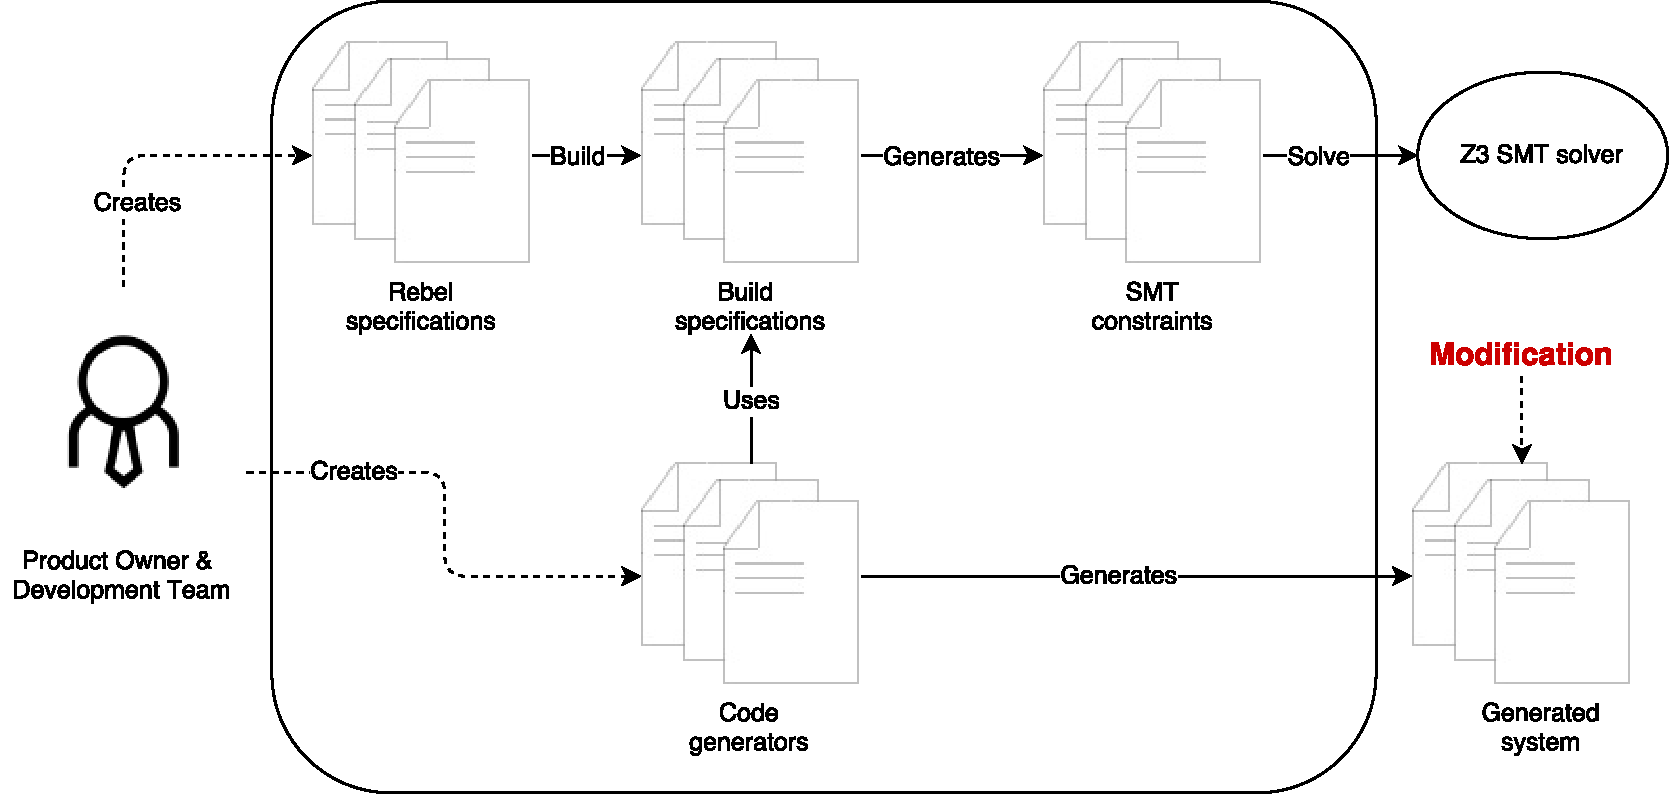
\includegraphics[width=\linewidth{}]{figures/modified-sut.pdf}
  \caption{Modification in specification development}\label{fig:mod-spec-gen}
\end{figure}
\FloatBarrier

\begin{sourcecode}[h!]
\begin{lstlisting}[language=scala]
case Close() => {
  RebelConditionCheck.success
}
\end{lstlisting}
\caption{Modified Precondition for \textit{close} event}\label{fig:account-close-mod-pre}
\end{sourcecode}
\FloatBarrier

\subsection{Evaluation criteria}\label{sec:ch4-eval-criteria}

\subsubsection{Bugs}
Since the precondition of the \textit{close} transition is modified in the \gls{sut},
we know that the \gls{sut} contains the bug to close an account with some balance. For
the lightweight version, it is expected to find this bug in the \gls{sut}.

\subsubsection{Efficiency}
The lightweight version will use checking to check whether it is possible to have
a closed account with some balance. Therefore, it is expected to test the same
transition in the \gls{sut}.

\subsubsection{Coverage}
With this lightweight version, we are going to trigger one single bug in the \gls{sut},
\textit{i.e.} finding the bug for the \textit{close} transition. Thus from the
account specification, we are testing only the transition \textit{close}.

\section{Approach}

\begin{figure}[h!]
  \centering
  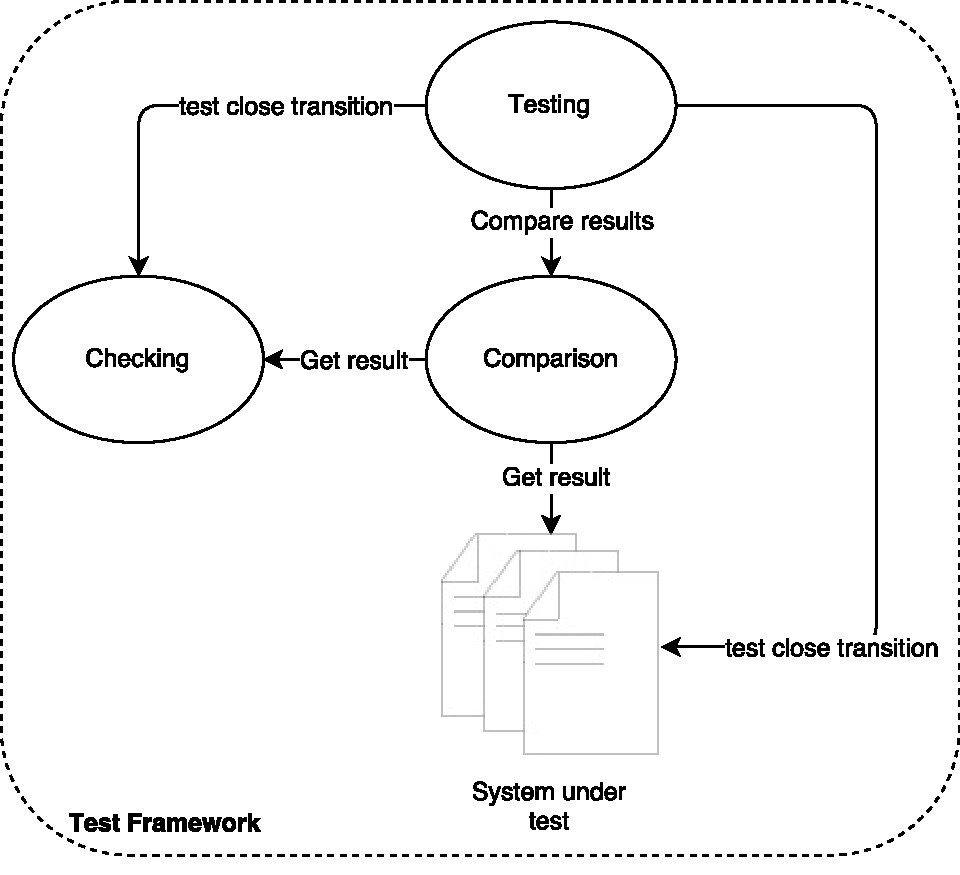
\includegraphics[width=\linewidth{}]{figures/test-modified-bug.pdf}
  \caption{Testing approach for \textit{close} transition}\label{fig:mod-bug-test}
\end{figure}
\FloatBarrier

The testing approach is shown in \autoref{fig:mod-bug-test}.
We discussed earlier that we are going to use the \gls{smt} solver to find bugs in the
\gls{sut}. Having an account with some balance in the state closed should not be possible
according to the specification. To let the \gls{smt} solver solve this situation, it
is necessary to generate the appropriate \gls{smt} formulas. Therefore, checking can
be used to check whether the given state with its properties is reachable.
The test framework first uses checking to test whether the state is reachable.

To check the state is a tebl file created which is shown in
\autoref{fig:tebl-closed-account}. It defines the state of a closed account with
the property balance, where the balance is not equal to zero. Also, here is six
used as configurable time-out. The \gls{smt} solver tries to solve this problem in
max six steps.

\begin{sourcecode}[h!]
\begin{lstlisting}[]
module simple_transaction.ClosedAccountWithBalance

import simple_transaction.Account

state closedAccountWithBalance {
  closed Account with balance != EUR 0.00;
}

check closedAccountWithBalance reachable in max 6 steps;
\end{lstlisting}
\caption{Closed account test}\label{fig:tebl-closed-account}
\end{sourcecode}
\FloatBarrier

The input for the \gls{smt} solver is now defined. Similar behaviour should be defined
for the \gls{sut}. So an account needs to be opened and closed
afterwards. Therefore, the testing framework performs both transitions in the
\gls{sut}.

The tebl file is passed to the model checker, and it returns whether the given
\gls{smt} problem is reachable or not. A state is reachable when it can be reached
from the initial state via valid
transitions.~\cite[p.~4]{stoel_storm_vinju_bosman_2016} To check if the state is
reachable in the \gls{sut}, the request made for the given transition
contains afterwards a check whether the request is successful. Then the testing
framework can compare the results from the \gls{smt} solver and the request made in
the \gls{sut}.

\section{Results}

\subsection{Codegen-Akka}

Since we have defined the input for both systems and can compare it, we
can trigger the bug and compare the results of it. The results of testing the
\textit{close} transition are shown in \autoref{fig:ch3-res-codegenakka-account}.

\begin{table}[h!]
\centering
\begin{tabular}{cccc}
\toprule
\textbf{Transition to test} & \textbf{Reachability \gls{smt} solver} & \textbf{Reachability \gls{sut}} & \textbf{Test result} \\ \midrule
close                       & \xmark{}                         & \cmark{}                  & \xmark{}             \\ \bottomrule
\end{tabular}
\caption{Results: testing \textit{close} transition of account specification}\label{fig:ch3-res-codegenakka-account}
\end{table}
\FloatBarrier

\section{Analyse}

\subsection{Codegen-Akka}
According to the results from \autoref{fig:ch3-res-codegenakka-account}, the
generated test for the \textit{close} transition has failed. The results of the
model checker state that the defined state in \autoref{fig:tebl-closed-account}
is not reachable. Although, the state in the \gls{sut} is reachable.

Looking at the account in the \gls{sut}, it looks as follows
\autoref{fig:mod-closed-account-json}. The state of the account is closed, and
the balance is the same as when it was opened. To conclude, the \textit{close}
transition is performed in the \gls{sut} due to the modification of the generated
precondition.

\begin{sourcecode}[h!]
\begin{lstlisting}[]
{
   "state":{
      "SpecificationState":{
         "state":{
            "Closed":{

            }
         }
      }
   },
   "data":{
      "Initialised":{
         "data":{
            "accountNumber":null,
            "balance":"EUR 50.00"
         }
      }
   }
}
\end{lstlisting}
\caption{Account state after \textit{close} transition}\label{fig:mod-closed-account-json}
\end{sourcecode}
\FloatBarrier

\section{Evaluation}\label{sec:ch3-evalution}

\subsubsection{Bugs}
The expectation for the bugs criteria is to find the bug in the \textit{close} transition.
As expected, we did find the bug for the \textit{close}
transition due to the manually modified precondition.

\subsubsection{Efficiency}

Checking is used in this lightweight version to check whether it is possible
to have an opened account with some balance. According to
\autoref{fig:ch3-res-codegenakka-account}, this state is not reachable. It is
expected to test the same transition with checking in the \gls{sut}.

When the model checkers returns that a given state is not reachable,
traces are not available. Models (traces) are not available when "unsat" is
returned by Z3.
In this case, traces cannot be used since they are not provided. Although, to
reach the given state are the \textit{openAccount} and \textit{close} transition
used.

\info{add reference for no model when unsat}

\subsubsection{Coverage}
The lightweight version is used only to trigger a single bug in the \gls{sut}. As
expected, only the transition \textit{close} tested. Although, to close an
account the account needs to be first opened. Therefore, the transition
\textit{openAccount} performed, but this transition is not tested whether the
request is successful.

\section{Conclusion}

As we have seen with this lightweight version, it can find one specific bug with the use of an \gls{smt} solver. Since the code generator is template based, it is possible to find faults in templating. There are two parts where there can occur faults during the generation parts. As described in~\cite[p.~274]{voelter2013dsl}, the majority of the generated code is fixed, some isolated parts are dependent on the input of the model. So it is possible that there might be bugs in the fixed code. The second part is the template control code which is injected into the generated code. The manually introduced bug from the previous chapter belongs  to this category.

\unsure{\textbf{Onduidelijkheid DSL fowler}: styles of code generation: Model-Aware Generation and Model Ignorant Generation. Styles for generating textual output: Transformer
Generation and Templated Generation.}

\info{transactions, atomic commits, consistency. <- dit is moeilijk te doen. welke bugs verwacht je? het is moeilijk iets te generate. en uitleggen waarom het moeilijk is testen.}
